\documentclass[border=10pt]{standalone}

\usepackage{tikz}
\usepackage{tikzsymbols}
\usetikzlibrary{calc,patterns,shapes.geometric}

\def\centerarc[#1](#2)(#3:#4:#5){\draw[#1] ($(#2)+({#5*cos(#3)},{#5*sin(#3)})$) arc (#3:#4:#5);}

\begin{document}
	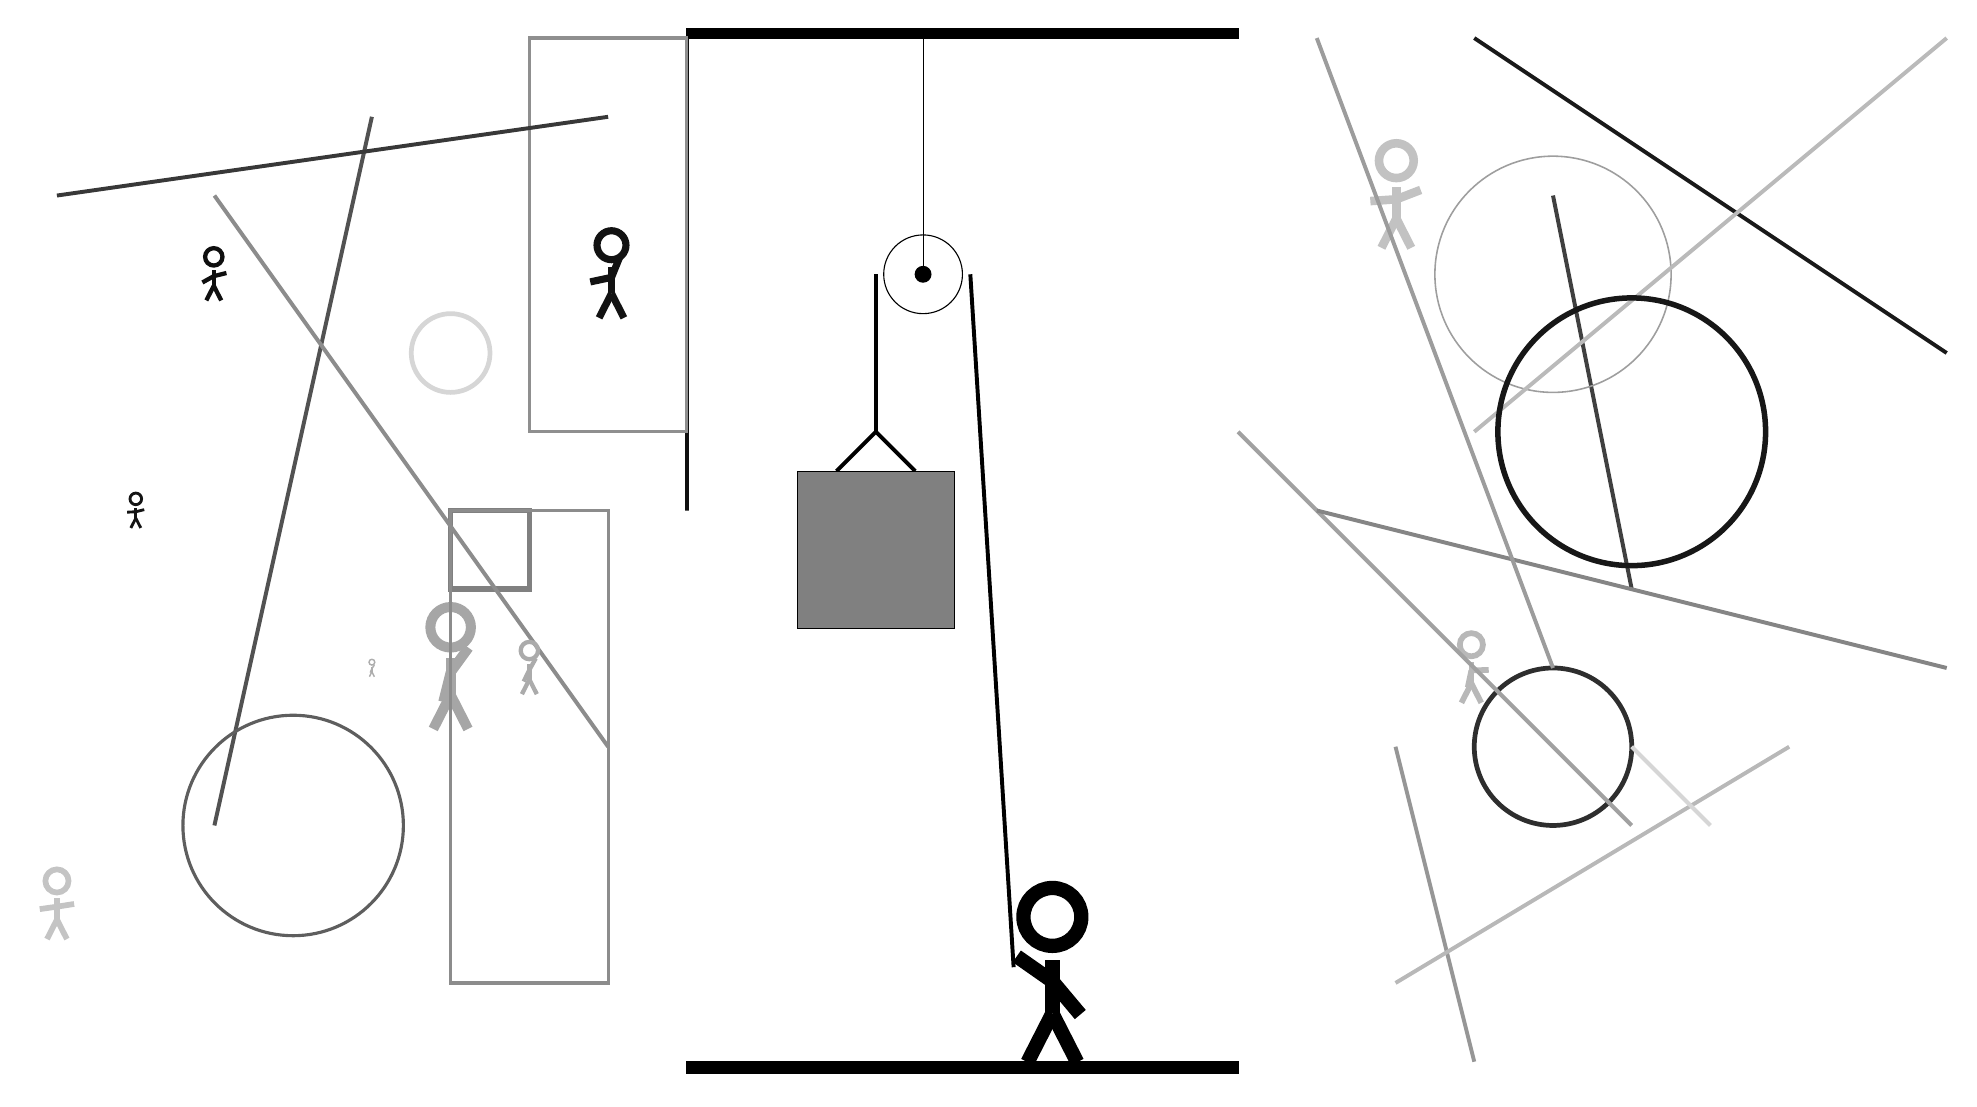
\begin{tikzpicture}
		%%%%% START %%%%%
		
		\draw[fill=black] (-2, 10) rectangle (5, 10.125);
		
		\draw (1, 7) circle (0.5);
		\draw[fill=black] (1, 7) circle (0.1);
		\draw (1, 10) -- (1, 7);
		
		\draw[line width=0.5mm] (-0.1, 4.5) -- (0.4, 5.0) -- (0.9, 4.5);
		\draw[fill=black!50] (-0.6, 4.5) rectangle (1.4, 2.5);
		
		\draw[line width=0.5mm, color=black!94] (-2, 10) rectangle (-2, 4);
		
		\draw[line width=0.7mm, color=black!50] (-4, 3) rectangle (-5, 4);
		\node[line width=0.7mm, color=black!32] at (-6, 2) {\Strichmaxerl[1][67][56]};
		\draw [line width=0.6mm, color=black!82](9, 1) circle (1.0);
		
		\draw[line width=0.5mm, color=black!68](-6, 9) -- (-8, 0);
		\draw [line width=0.4mm, color=black!63](-7, 0) circle (1.4);
		
		\node[line width=0.3mm, color=black!35] at (-5, 2) {\Strichmaxerl[7][76][54]};
		\node[line width=0.5mm, color=black!28] at (8, 2) {\Strichmaxerl[4][78][2]};
		\node[line width=0.3mm, color=black!92] at (-9, 4) {\Strichmaxerl[2][3][14]};
		\draw[line width=0.5mm, color=black!90](8, 10) -- (14, 6);
		\node[line width=0.5mm, color=black!24] at (7, 8) {\Strichmaxerl[6][4][21]};
		\draw[line width=0.5mm, color=black!45](-3, 1) -- (-8, 8);
		\draw[line width=0.4mm, color=black!44] (-4, 5) rectangle (-2, 10);
		\draw[line width=0.5mm, color=black!37](10, 0) -- (5, 5);
		\draw [line width=0.6mm, color=black!16](-5, 6) circle (0.5);
		\node[line width=0.5mm, color=black!93] at (-3, 7) {\Strichmaxerl[5][12][68]};
		
		\draw[line width=0.5mm, color=black!41](7, 1) -- (8, -3);
		
		\draw[line width=0.5mm, color=black!78](-3, 9) -- (-10, 8);
		\draw[line width=0.4mm, color=black!45] (-3, 4) rectangle (-5, -2);
		
		\draw[line width=0.5mm, color=black!75](9, 8) -- (10, 3);
		\draw[line width=0.5mm, color=black!28](7, -2) -- (12, 1);
		\draw[line width=0.5mm, color=black!48](6, 4) -- (14, 2);
		\draw [line width=0.2mm, color=black!38](9, 7) circle (1.5);
		\node[line width=0.2mm, color=black!94] at (-8, 7) {\Strichmaxerl[3][29][14]};
		\draw[line width=0.5mm, color=black!27](8, 5) -- (14, 10);
		\draw [line width=0.7mm, color=black!91](10, 5) circle (1.7);
		
		\node[line width=0.7mm, color=black!23] at (-10, -1) {\Strichmaxerl[4][8][9]};
		\draw[line width=0.5mm, color=black!39](6, 10) -- (9, 2);
		\draw[line width=0.5mm, color=black!16](10, 1) -- (11, 0);
		
		\node[line width=0.2mm, color=black!33] at (-4, 2) {\Strichmaxerl[3][64][61]};
		
		\draw[line width=0.5mm] (0.4, 7) -- (0.4, 5.0);
		\centerarc[line width=0.5mm](1, 7)(0:180:0.6);
		\draw[line width=0.5mm](1.6, 7) -- (2.15, -1.8);
		
		\node at (2.6, -1.9) {\Strichmaxerl[10][-35][-50]};
		
		\draw[fill=black] (-2, -3) rectangle (5, -3.15);
		
		%%%%% END %%%%%
	\end{tikzpicture}
\end{document}